\chapter{Results}
In this chapter the results of multiple runs of the program will be discussed, both in 2D and 3D. First some runs in 2D will be discussed along with how the variables in the speed function affects the segmentation. Then some results from 3D runs will be illustrated, before the performance of different runs are compared. The Chan-Vese speed function implemented will not be discussed in any detail because the very simplified version implemented behaves much like a simple region grow function.

A note about the values used to get the segmentation results in this chapter, the values used for the speed function were found to give a good result when manually comparing to the input images/volumes, and may or may not be the optimal values for speed and accuracy. Also note that the colors used in the volumes are only to illustrate the difference in number of iterations, and the colors for the same number of iterations vary from figure to figure.

\section{2D}
First a simple binary image of size 512x512 of a circle shown in figure \ref{circleZeroMany}a was segmented. The red dot in the middle represents the seed point chosen, and is not part of the image (superimposed). The values used for the speed funcition were: threshold ($T$) = 0.99, $\epsilon$ = 0.15 and $\alpha$ = 0.80. Since this image is binary the $T \pm \epsilon$ would not affect the end result of a full segmentation, as long as $T - \epsilon < 1 < T + \epsilon$. This also assumes that $T - \epsilon$ is not too close to 0, which would (also depending on $\alpha$) either stop the surface evolution midways or collaps it. The advantage of using higher values of $\epsilon$ within these limits is that higher values of $\epsilon$ makes the segmentation process faster by needing less iterations to achieve full segmentation. The reason is that the data term $D(I)$ (see \ref{dataFunction}) in the speed function is gradual, as mentioned when describing the speed function in chapter \ref{levelSetChap}.

Figures \ref{circleZeroMany} b, c and d represents the zero level set after 700, 1200 and 1600 iterations respectively. Figure \ref{circleZeroMany}d illustrates the full segmentation result which required 2200 iterations.

\begin{figure}[h!]
\centering
\begin{minipage}{.49\textwidth}
\begin{tabular}{c}

\includegraphics[width=0.95\textwidth]{results/2D/circle} \\
(a)
\end{tabular}
\end{minipage}
\begin{minipage}{.49\textwidth}
\begin{tabular}{c}

\includegraphics[width=.9\textwidth]{results/2D/circleZero700} \\
(b)
\end{tabular}
\end{minipage}
\\
\begin{minipage}{.49\textwidth}
\begin{tabular}{c}
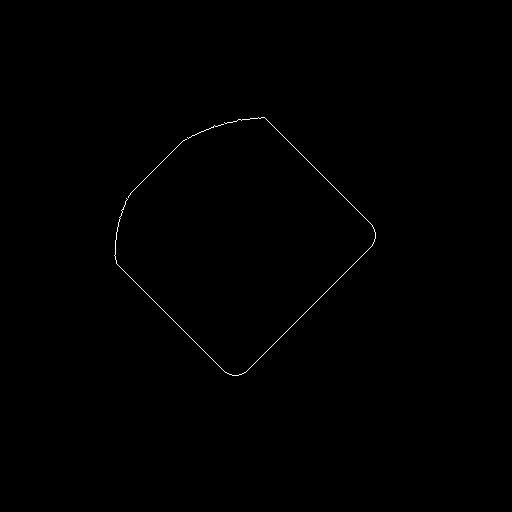
\includegraphics[width=.9\textwidth]{results/2D/circleZero1200} \\
(c)
\end{tabular}
\end{minipage}
\begin{minipage}{.49\textwidth}
\begin{tabular}{c}
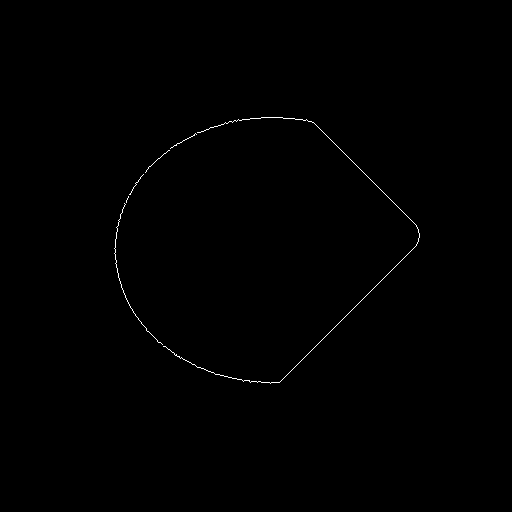
\includegraphics[width=.9\textwidth]{results/2D/circleZero1600} \\
(d)
\end{tabular}
\end{minipage}
\\
\begin{minipage}{.49\textwidth}
\begin{tabular}{c}
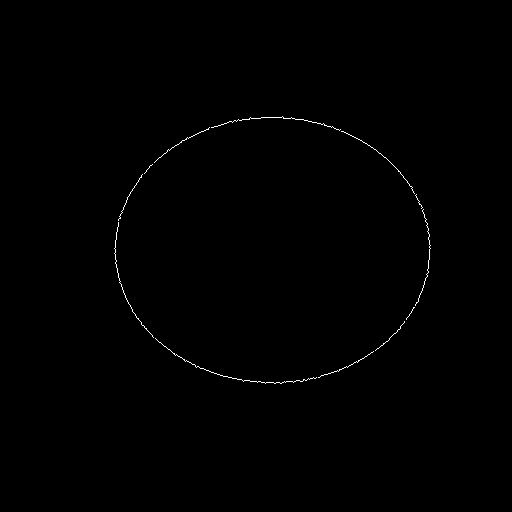
\includegraphics[width=.9\textwidth]{results/2D/circleZero2200_full} \\
(e)
\end{tabular}
\end{minipage}
\begin{minipage}{.49\textwidth}
\begin{tabular}{c}

\includegraphics[width=.9\textwidth]{results/2D/circleEps005} \\
(f)
\end{tabular}
\end{minipage}
\caption{(a): Original image with seed point. Zero level set after: (b): 600, (c): 1200, (d): 1600 and (e): 2200 iterations (e): with $\epsilon=0.05$.}
\label{circleZeroMany}
\end{figure}
\clearpage

By comparing the input image in figure \ref{circleZeroMany}a with the segmentation result in figure \ref{circleZeroMany}e it can be seen that the program succesfully segmented the image. To measure the difference in iterations needed to get a full segmentation with a different value of $\epsilon$ an additional segmentation with all variables equal to the previous segmentation except for $\epsilon$ was performed. By assigning $\epsilon$ a value 0.05 the result was the exact same after full segmentation, but the numbers of iterations for full segmentation increased by nearly four times, from 2200 to about 8600. By omparing figure \ref{circleZeroMany}e with figure \ref{circleZeroMany}f which is the result after 2200 iterations with $\epsilon$ = 0.05 it can be seen how much slower the interface evolves.

To test if the program works as it should when parts of the seed point is outside the object to be segmented, the seed point was set as shown in red in figure \ref{circleSeedPartlyOutside}a. How the interface looked like after 300, 800 and 1300 iterations is depicted in figure \ref{circleSeedPartlyOutside}b, c and d respectively. The final segmentation result was as expected a correct segmentation of the object as in figure \ref{circleZeroMany}e. 
\begin{figure}[h!]
\centering
\begin{minipage}{.49\textwidth}
\begin{tabular}{c}
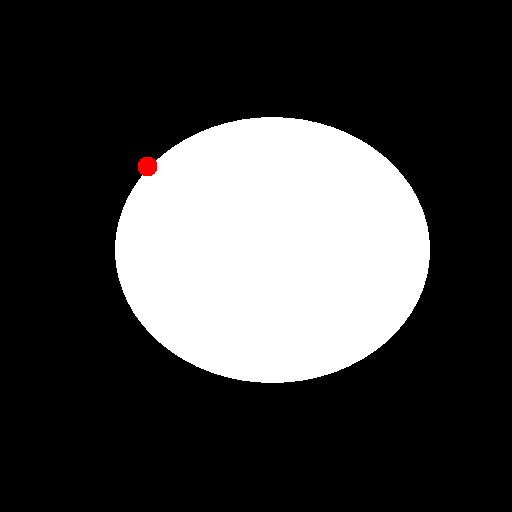
\includegraphics[width=.9\textwidth]{results/2D/circleSeedPartlyOutside} \\
(a)
\end{tabular}
\end{minipage}
\begin{minipage}{.49\textwidth}
\begin{tabular}{c}
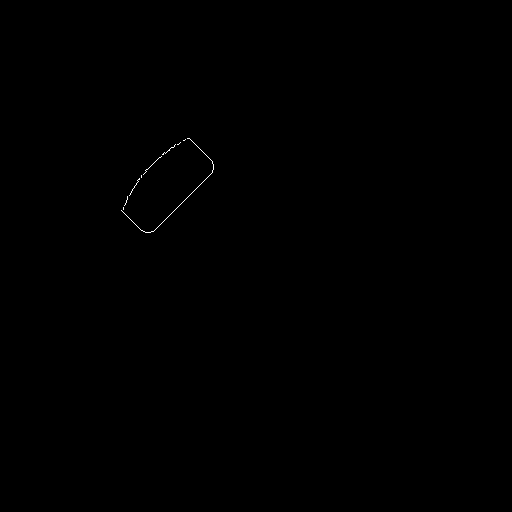
\includegraphics[width=.9\textwidth]{results/2D/circleSeedPartlyOutside300} \\
(b)
\end{tabular}
\end{minipage}
\\
\begin{minipage}{.49\textwidth}
\begin{tabular}{c}
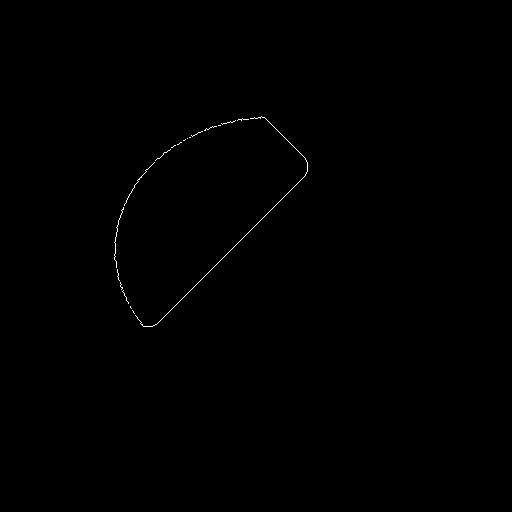
\includegraphics[width=.9\textwidth]{results/2D/circleSeedPartlyOutside800} \\
(c)
\end{tabular}
\end{minipage}
\begin{minipage}{.49\textwidth}
\begin{tabular}{c}
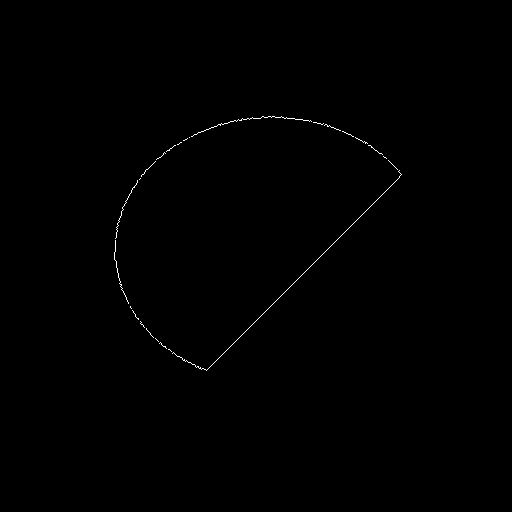
\includegraphics[width=.9\textwidth]{results/2D/circleSeedPartlyOutside1300} \\
(d)
\end{tabular}
\end{minipage}
\caption{(a): Seed point partly outside the object, superimposed on the input image. Interface after (b): 300, (c): 800 and (d): 1300 iterations.}
\label{circleSeedPartlyOutside}
\end{figure}

To further test the robustness of the program and to illustrate the effect $\alpha$ has on the smoothness of the interface the 512x512 binary image in figure \ref{randOrgWSeed}a, with the seed point superimposed in red, was segmented. Notice the one-pixel wide "cut" at the top that seperates the main object in the image from the smaller one. Also notice the one-pixel wide line that holds together the main object with the rectangle at the button. Two full segmentations were run, both with $T$ = 0.99 and $\epsilon$ = 0.15, figure \ref{randOrgWSeed}b is the result with $\alpha$ = 0.80 and \ref{randOrgWSeed}c with $\alpha$ = 0.90.
\begin{figure}[h!]
\centering
\begin{minipage}{.46\textwidth}
\begin{tabular}{c}
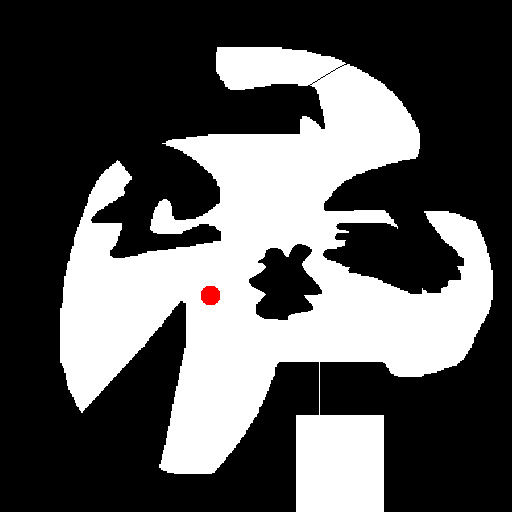
\includegraphics[width=.9\textwidth]{results/2D/randOrgWSeed} \\
(a)
\end{tabular}
\end{minipage}
\\
\begin{minipage}{.46\textwidth}
\begin{tabular}{c}
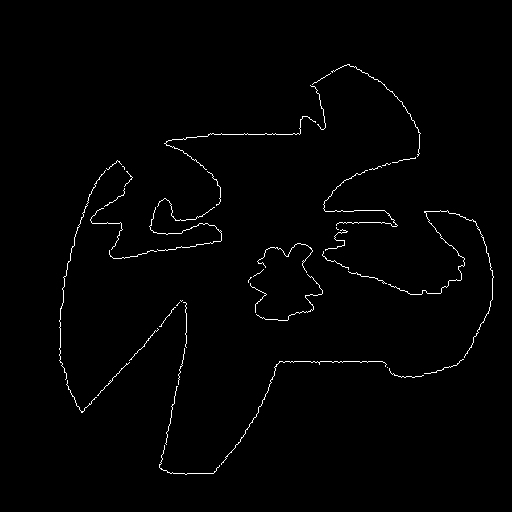
\includegraphics[width=.9\textwidth]{results/2D/randOrgWSeeda080} \\
(b)
\end{tabular}
\end{minipage}
\begin{minipage}{.46\textwidth}
\begin{tabular}{c}
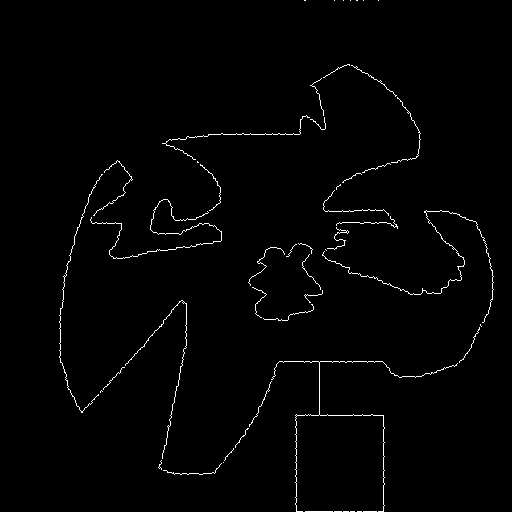
\includegraphics[width=.9\textwidth]{results/2D/randOrgWSeeda090} \\
(c)
\end{tabular}
\end{minipage}
\caption{(a): Input image with seed point superimposed. Segmentation result with (b): $\alpha$ = 0.80, (c): $\alpha$ = 0.90.}
\label{randOrgWSeed}
\end{figure}
As explained in chapter \ref{levelSetChap}, $\alpha$ restricts how much the interface can bend and prevents the model from leaking into unwanted areas, which can be seen by the fact that \ref{randOrgWSeed}c with a higer value of $\alpha$ have been able to include the rectangle at the button by evolving through the thin line, while \ref{randOrgWSeed}b with only a value of 0.10 $\alpha$ less did not manage it. Higher values gives more importance to \(D(I)\) and lower values makes \(\nabla \frac{\nabla \phi}{|\nabla \phi|}\) affect the level set more. The more importance \(\nabla \frac{\nabla \phi}{|\nabla \phi|}\) gets, the less likely is the model to leak into unwanted areas. But giving \(\nabla \frac{\nabla \phi}{|\nabla \phi|}\) too much importance makes the model so smooth that it does not reach all areas of the object being segmented. This is illustrated in figure \ref{starZero}b, which is the segmentation result of the image in figure \ref{starZero}a using $\alpha$ = 0.4. To clearly illustrate the effects of $\alpha$ on the smoothness of the segmentation result, figures \ref{starZero}a and b are small of size (100x100).
\begin{figure}[h!]
\centering
\begin{minipage}{.35\textwidth}
\begin{tabular}{c}

\includegraphics[width=.9\textwidth]{results/2D/starZero} \\
(a)
\end{tabular}
\end{minipage}
\begin{minipage}{.35\textwidth}
\begin{tabular}{c}

\includegraphics[width=.9\textwidth]{results/2D/starZeroFullSeg} \\
(b)
\end{tabular}
\end{minipage}
\caption{Interface smoothness highly valued. (a): Input image, (b): segmentation result.}
\label{starZero}
\end{figure}
\clearpage

\section{3D}
First volume to be segmented is a volume of an aneurism in a "semi segmented brain volume". 
\begin{figure}[h!]
\centering
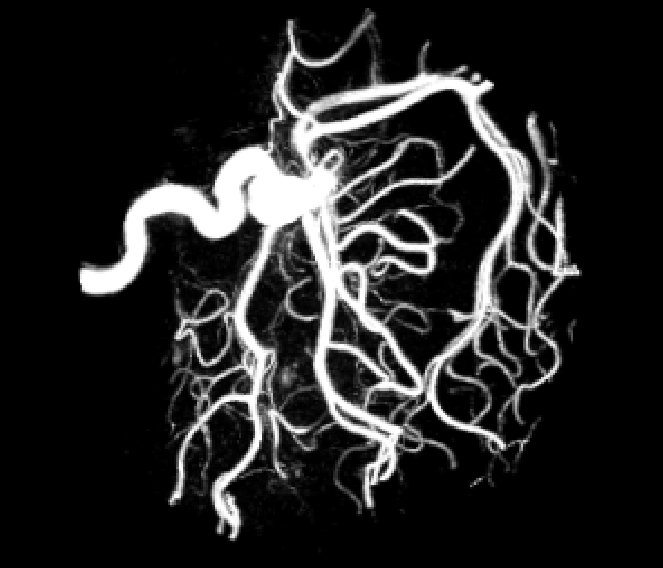
\includegraphics[width=.9\textwidth]{results/3D/3D-aneurism-unsegmented/aneurism_original_mip}
\caption{Maximum intensity projection of the volume to be segmented}
\label{aneurismOriginal}
\end{figure}
The goal is to segment the aneurism itself as well as adjacent connected arteries without expanding into insignificant parts of the volume. In figure \ref{aneurismOriginal} the maximum intensity projection of the unsegmented volume is depicted. 

Figure \ref{aneurism500iterations} shows how the segmented image looks like after 500 iterations. The values used are $T$ = 1.0, $\epsilon$ = 0.3 and $\alpha$ = 0.75. 
\begin{figure}[h!]
\centering
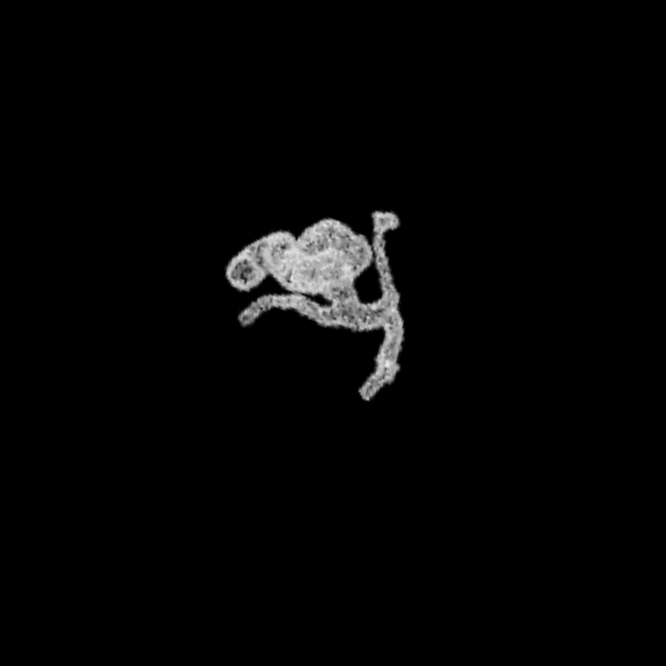
\includegraphics[width=.9\textwidth]{results/3D/aneurism_500_iterations}
\caption{Aneurism segmentation after 500 iterations.}
\label{aneurism500iterations}
\end{figure}
The dimension of the aneurism volume is 256x256x256 and the maximal expanding speed the interface can have using the implemented speed funciton is 1 pixel per iteration. In theory this would mean that only about half the number of iterations of the greatest image dimension is needed (assuming the seed point is located near the center of the volume) in order to achieve convergence. But this assumes an average speed of 1 pixel per iteration, which in practice does not happen. The speed is reduced by both the curcature of the object being segmented and the intensity values of the neighbouring pixels. And in this case, whith an aneurism volume with narrow paths, the curvature greatly reduces the speed of the evalution process. It turns out that to achieve a satisfying result of the aunerism volume with the given the input parameters stated above, about 3000 iterations is needed. 
\begin{figure}[h!]
\centering
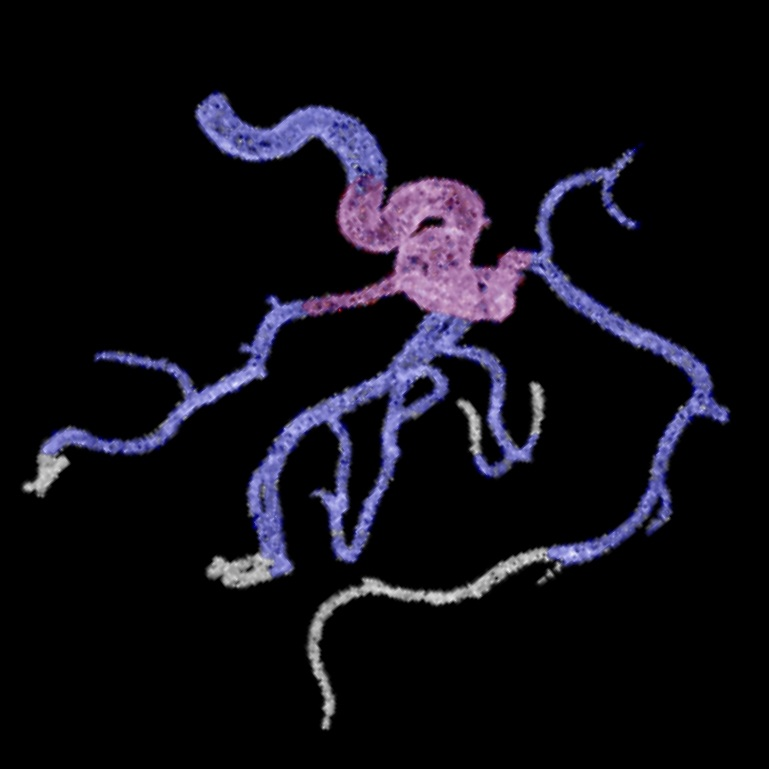
\includegraphics[width=.9\textwidth]{results/3D/aneurism_3000_1500__500_iter}
\caption{Aneurism segmentation after 500 (red), 1500 (blue) and 3000 (gray) iterations.}
\label{aneurism30001500500iter}
\end{figure}

Figure \ref{aneurism30001500500iter} shows the segmentated volume after 500, 1500 and 3000 iterations. The red part of the structure is the result of the segmentation after 500 iterations (same as in figure \ref{aneurism500iterations}). The light blue colored part shows the segmentation after 1500 iterations and the gray colored part is the result after 3000 iterations. The figure shows how stable the algorithm is throughout the run. The area along the walls of the arteries covered after 500 iterations is not retracting at a later point, nor is it expanding further. This is shown by observing how well the 500 iterations volume and the 1500 iterations volume overlap.

%3000_2000 bilde her kanskje?

Next, the original volume (not MIP as in figure \ref{aneurismOriginal}) in gray is compared to the result after 3000 iterations (in blue). The completely gray arteries are not connected to the aneurism where the seed point was set and are thus not reachable unless additional seed points are set at their locations. But apart from those arteries it can be seen that the segmentation result have been able to access the majority of the arteries, except for a few locations (e.g. at the top right corner) which was too narrow for the level set to access given the current values used in the speed funcion. Some segmentations given different values were executed to access these areas, but that resulted in the level set leaking into other areas not connected to the seed location.
\begin{figure}[h!]
\centering
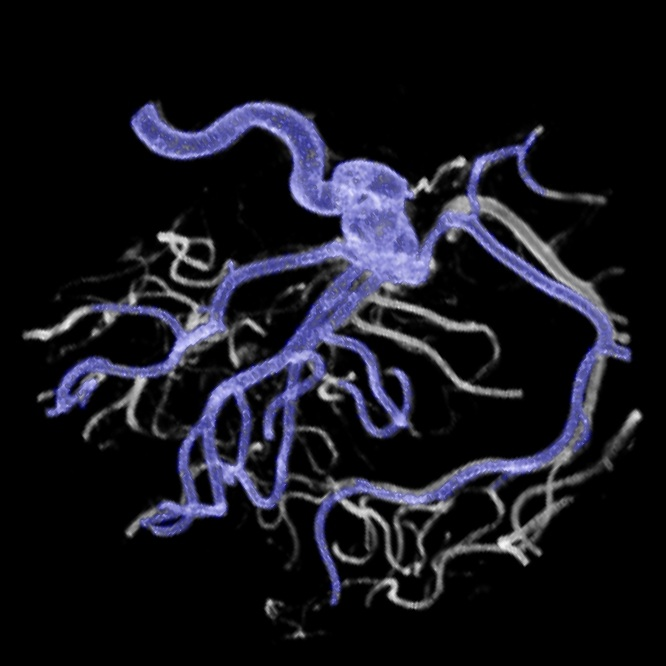
\includegraphics[width=.9\textwidth]{results/3D/aneurism_orginal_3000_iter}
\caption{Aneurism: original volume in gray and segmentation result after 3000 iterations in blue.}
\label{aneurismorginal3000iter}
\end{figure}

By looking at all the aneurism segmentation results above it can be seen how good the implemented version of the sparse field level set metod is to expand through narrow paths without leaking outside the segmentation object given the correct speed function values.

A T1-weighted MRI volume of a head was segmented to extract out the brain. The head volume along with the segmentation result of the brain (in red) is illustrated in figure \ref{brainT14000itst024e009a065}. The number of iterations needed to achieve this result was 4000, and the values used are $T$ = 0.24, $\epsilon$ = 0.09 and $\alpha$ = 0.65. Figure \ref{brainSegSlicees}a and b illustrates the segmentation result as a superimposition on the original volume along different coordinates of the z-axis.
\begin{figure}[h!]
\centering
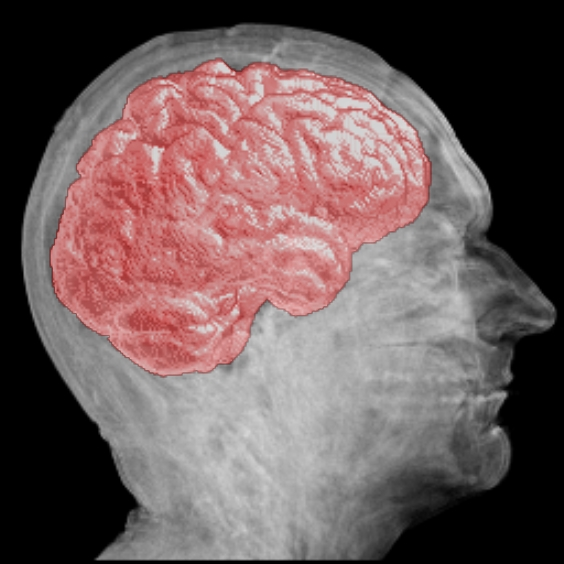
\includegraphics[width=.9\textwidth]{results/3D/brainT1_4000_its_t024e009a065}
\caption{Original volume of head and segmented brain volume in red.}
\label{brainT14000itst024e009a065}
\end{figure}

\begin{figure}[h!]
\centering
\begin{minipage}{.35\textwidth}
\begin{tabular}{c}

\includegraphics[width=.9\textwidth]{results/2D/starZero} \\
(a)
\end{tabular}
\end{minipage}
\begin{minipage}{.35\textwidth}
\begin{tabular}{c}

\includegraphics[width=.9\textwidth]{results/2D/starZeroFullSeg} \\
(b)
\end{tabular}
\end{minipage}
\caption{Slices along the z-axis of the brain segmented volume, superimposed on the original volume.}
\label{brainSegSlicees}
\end{figure}

The program was also tested on a CT volume of an abdomen by to extracting out the volume of the liver. This process is somewhat tricky because the liver has greyscale values very similar to the organs surrounding it, making it difficult to prevent the interface from leaking into the surroundings. Although the curvature term will prevent pixel sized leaks and small holes, it will not prevent a broad part of the interface to move out of the liver volume unless the curvatures is weighted heavily. In addition, the internal structures of the liver migh vary even more than the liver and its surroundings. So the parameters has to be chosen wisely to get a good segmentation. Figure \ref{CTliverZaxis} (TODO: lag bildet) shows a slice in the z-axis of the volume. The liver is the big semi-uniform area that stretches from the left and over the middle of the stomach. As we can see the difference in the pixel values between the liver area and its surroundings are small. The dimensions of the image are 320x220x72. Next we see the segmented volume (figure ct with poor threshold) using values (insert values for liver CT) and (insert iterations) iterations. The threshold in this image (reference figure ct with poor threshold) is too high and so the 
%\begin{figure}[h!]
%\centering
%\includegraphics[width=.9\textwidth]{results/3D/CTliverZaxis}
%\caption{Slice of CT liver volume in the z-axis.}
%\label{CTliverZaxis}
%\end{figure}
%TODO: lag bildet CTliverZaxis

\section{Performance}
\subsection*{Testing environment}
The tests were performed on a laptop PC with the specifications as described in table \ref{pcSpecs}. The software related specifications are Windows 7 as operative system, g++ version 4.6.2 as C++ compiler, and CUDA compute capability 5.0 with nvcc version 0.2.1221 as compiler.

\begin{table}[h!]
	\begin{tabular}{| c | c |} 
	\hline
	\multicolumn{2}{|c|}{PC the tests were executed on} \\
	\hline
	CPU model & Intel Core i5-320M \\
	\hline
	Cores in CPU & 2 \\
	\hline
	CPU frequency & 2.5GHz \\
	\hline
	Memory & 4GB \\
	\hline
	GPU model & NVIDIA GeForce GT 630M \\
	\hline
	Cores in GPU & 96 \\
	\hline
	GPU memory & 1GB \\
	\hline
	\end{tabular}
	\caption{Specifications of the PC the tests were performed on.}
	\label{pcSpecs}
\end{table}


 
TODO 
HELT til slutt i kapittelet: en tabell med antall iterasjoner og tid brukt på alle segmenteringene, både 2D og 3D (eventuelt også CUDA). The results in this table were all aquired by using a single seed point set at an optimal location close to the center of the object being segmented, with a radius of 10. The variable values used were found to be the fastest ones, given a specific object, while resulting in a correct and complete segmentation. The time was taken for only the segmentation process, thus not including the time used to read input, initialize and write result back to file.